\documentclass{article}

% Remove all section numbers everywhere
\setcounter{secnumdepth}{0}

\newcommand{\st}{\textsuperscript{st}}
\newcommand{\nd}{\textsuperscript{nd}}
\newcommand{\rd}{\textsuperscript{rd}}
\renewcommand{\th}{\textsuperscript{th}}


\usepackage[margin=1in]{geometry}
\usepackage{accessibilityMeta}
\usepackage{multicol}
\usepackage{verbatim}
\usepackage{caption}
\usepackage[dvipsnames]{xcolor}
\usepackage{pgfplots}
\usepackage{pgfplotstable}
\pgfplotsset{compat=newest}

\usepackage{titlesec}
\newcommand{\sectionbreak}{\clearpage}

\usepackage{tikz}
\usepackage{pgf-pie}
\newcommand{\pieslicecaption}[3]{{#1, \dollar{#2}, \SI{#3}{\percent}}}

\usepackage{siunitx}
% Configure siunitx for money
\sisetup{
  group-four-digits = true,
  group-separator = {,}
}

% Define helper for writing money: \dollar{4}
\newcommand{\dollar}[1]{\SI{#1}[\$]{}}
\newcommand{\trydollar}[1]{
	\ifnum9<1#1\relax\dollar{#1}
	\else
		#1
	\fi
}

\usepackage{intcalc}
\usepackage{xstring}
\usepackage{enumerate}
\usepackage{enumitem}
\usepackage{ifthen}
\usepackage{xparse}
\usepackage{etoolbox}

\newcounter{goal}[section] % section isn't resetting :(
\pretocmd{\section}{\setcounter{goal}{0}}{}{} % https://tex.stackexchange.com/questions/264335/when-using-section-counters-dont-reset-properly-how-to-fix-this

\makeatletter
\DeclareDocumentCommand{\Goal@Goal}{o}{
	\stepcounter{goal}
	\subsection{Goal \arabic{goal}\IfNoValueF{#1}{ (#1)}}
}
\newcommand{\Goal@desc}[1]{
	\begin{quotation}
		#1
	\end{quotation}
}
\newcommand{\Goal@priorities}[2]{
	\subsubsection{State and/or Local Priorities addressed by this goal:}
	\begin{quote}
		\begin{itemize}[label={}]
			\item State Priorities: #1
			\item Local Priorities: #2
		\end{itemize}
	\end{quote}
}
\newcommand{\Goal@need}[1]{
	\subsubsection{Identified Need:}
		\begin{quotation}
			#1
		\end{quotation}
}
\DeclareDocumentCommand{\Goal}{o m m m g}{
	\Goal@Goal[#1]
	\Goal@desc{#2}
	\Goal@priorities{#3}{#4}
	\IfNoValueF{#5}{\Goal@need{#5}}
}

% Define Expected:/Actual: alternating enumeration labels.
% Use \begin{enumerate}[label=\expact]
\newcommand*{\expact}[1]{%
	\expandafter\@expact\csname c@#1\endcsname%
}
\newcommand*{\@expact}[1]{%
% wrapped in $...$ and \text to compel align right
	$\ifcase\intcalcAdd{1}{\intcalcMod{\intcalcSub{#1}{1}}{2}}
		\or{\text{Expected:}}
		\or{\text{Actual:}}
    \else\@ctrerr\fi$
}
\AddEnumerateCounter{\expact}{\@expact}{Expected:}

% Define Expected Annual Measurable Outcome table heading enumeration labels.
% Use \begin{enumerate}[label=\expout]
\newcommand*{\expout}[1]{%
	\expandafter\@expout\csname c@#1\endcsname%
}
\newcommand*{\@expout}[1]{%
% wrapped in $...$ and \text to compel align right
	$\ifcase\intcalcAdd{1}{\intcalcMod{\intcalcSub{#1}{1}}{4}}
		\or{\text{Baseline:}}
		\or{\text{2017--18:}}
		\or{\text{2018--19:}}
		\or{\text{2019--20:}}
    \else\@ctrerr\fi$
}
\AddEnumerateCounter{\expout}{\@expout}{Baseline:}
\makeatother

\newcommand{\outcome}[2]{
	\item
	\begin{enumerate}[label=\expact*]
	\setlength{\itemsep}{0pt}
	\item #1
	\item #2
	\end{enumerate}
}

\newcommand{\expoutcome}[5]{
	\item
	{\em Metric/Indicator: #1}
	\begin{enumerate}[label=\expout*]
		\setlength\itemindent{40pt}
		\item #2
		\item #3
		\item #4
		\item #5
	\end{enumerate}
}
\newenvironment{outcomes}
	{
		\subsubsection{Annual Measurable Outcomes}
		\begin{itemize}[label={}]
	}
	{\end{itemize}}

\newenvironment{expoutcomes}
	{
		\subsubsection{Expected Annual Measurable Outcomes}
		\begin{itemize}[label={}]
	}
	{\end{itemize}}


\newcounter{action}[goal]

\newcommand{\actionupdate}[4]{
	\stepcounter{action}
	\paragraph{Action \theaction}
	\begin{itemize}[label={}]
		\item Planned Actions/Services: #1
		\item Actual Actions/Services: #2
		\item Budgeted Expenditures: 
			\trydollar{#3}
		\item Estimated Actual Expenditures: 
			\trydollar{#4}
	\end{itemize}
}

\makeatletter
\DeclareDocumentCommand{\planaction@scope}{m m g}{
	\begin{itemize}[label={}]
		\item {\bf Students to be Served:} #1
			%\IfBooleanTF{#1}{\item {\bf Scope of Services:} #3}{}
		\IfNoValueTF{#3}{
		\item {\bf Location(s):} #2
		}{
		\item {\bf Scope of Services:} #2
		\item {\bf Location(s):} #3
		}
	\end{itemize}
}
\DeclareDocumentCommand{\planaction@action}{m m m m m m}{
	\paragraph{Actions/Services}
	\begin{itemize}[label={}]
		\item 2017--18 (#1): #4
		\item 2018--19 (#2): #5
		\item 2019--20 (#3): #6
	\end{itemize}
}
\DeclareDocumentCommand{\planaction@budget@row}{m m m}{
	\begin{itemize}[label={}]
		\item Amount: \trydollar{#1}
		\item Source: #2
		\item Budget Reference: #3
	\end{itemize}
}
\DeclareDocumentCommand{\planaction@budget}{m m m m m m m m m}{
	\paragraph{Budgeted Expenditures}
	\begin{itemize}[label={}]
		\item Year: 2017--18
			\planaction@budget@row{#1}{#4}{#7}
		\item Year: 2018--19
			\planaction@budget@row{#2}{#5}{#8}
		\item Year: 2019--20
			\planaction@budget@row{#3}{#6}{#9}
	\end{itemize}
}
	
\DeclareDocumentCommand{\planaction}{s m}{
\item #2\newline
	\IfBooleanTF{#1}{Included}{Not included} as contributing to meeting the Increased or Improved Services Requirement.
}
\makeatother

\DeclareDocumentEnvironment{planactions}{o}
	{
		\subsubsection{Planned Actions/Services}
		\IfNoValueF{#1}{#1}
		\makeatletter
		\begin{enumerate}[label={\bf Action \theenumi:}]
	}
	{
		\end{enumerate}
		\makeatother
	}

% TODO: Consider porting to action counter, but might not be necessary
\newenvironment{actionanalysis}
	{
		\begin{enumerate}[label={\bf Action \theenumi:}]
	}
	{
		\end{enumerate}
	}

\DeclareDocumentEnvironment{demIISUP}{m m m}
	{
		\subsection{LCAP Year: #1}
		\begin{itemize}[label={}]
		\item Estimated Supplemental and Concentration Grant Funds: \trydollar{#2}
		\item Percentage to Increase or Improve Services: #3
		\end{itemize}
		Describe how services provided for unduplicated pupils are increased or improved by at least the percentage identified above, either qualitatively or quantitatively, as compared to services provided for all students in the LCAP year.

		Identify each action/service being funded and provided on a schoolwide or LEA-wide basis. Include the required descriptions supporting each schoolwide or LEA-wide use of funds (see instructions).
		\begin{quotation}
	}
	{
		\end{quotation}
	}
\DeclareDocumentCommand{\iisup}{m m}{
	\par{\bf #1 --\trydollar{#2}} 
}

\begin{document}

\section{LCFF Budget Overview for Parents}
\begin{itemize}[noitemsep,label={}]
\item Local Educational Agency (LEA) Name: Sherman Thomas STEM Academy
\item CDS Code: 20-65243-0134510
\item Local Control and Accountability Plan (LCAP) Year: 2019--20
\item LEA contact information: Jamie Brock, 559-871-5490, jabrock@stcsca.org
\end{itemize}

School districts receive funding from different sources: state funds under the Local Control Funding Formula (LCFF), other state funds, local funds, and federal funds. LCFF funds include a base level of funding for all LEAs and extra funding---called ``supplemental and concentration'' grants---to LEAs based on the enrollment of high needs students (foster youth, English learners, and low-income students).

\subsection{Budget Overview for the 2019-20 LCAP Year}
\begin{figure}[hbtp]
\centering
Projected Revenue by Fund Source
	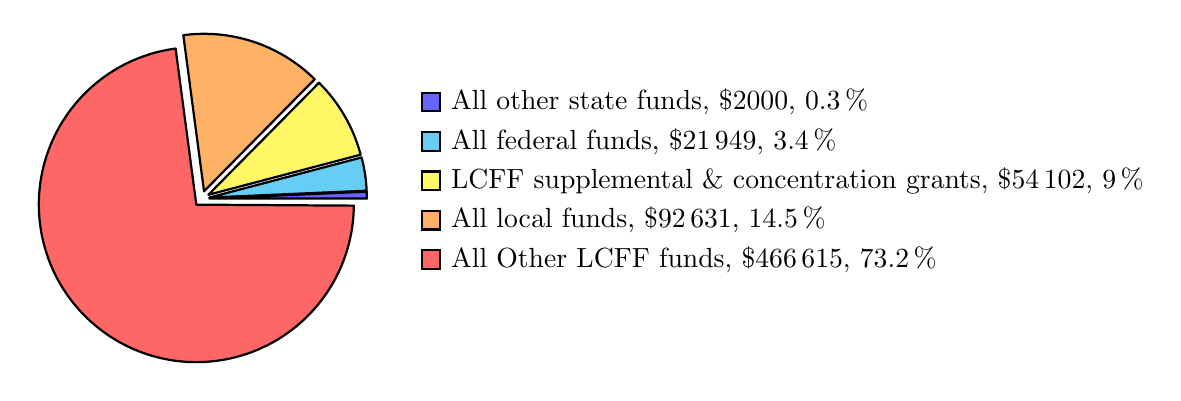
\begin{tikzpicture}
	\pie[explode=0.1, radius=2, rotate=0, text=legend, before number=\phantom, after number=]{
		  0.7/\pieslicecaption{All other state funds}{2000}{0.3},
		  3.4/\pieslicecaption{All federal funds}{21949}{3.4},
		  8.5/\pieslicecaption{LCFF supplemental \& concentration grants}{54102}{9},
		 14.5/\pieslicecaption{All local funds}{92631}{14.5},
		%81.7/\pieslicecaption{Total LCFF funds}{520717}{81.7},
		 72.8/\pieslicecaption{All Other LCFF funds}{466615}{73.2}
	}
	\end{tikzpicture}
	\caption*{This chart shows the total general purpose revenue Sherman Thomas STEM Academy expects to receive in the coming year from all sources.}
\end{figure}

The total revenue projected for Sherman Thomas STEM Academy is \dollar{637297.00}, of which \dollar{520717.00} is Local Control Funding Formula (LCFF), \dollar{2000.00} is other state funds, \dollar{92631.00} is local funds, and \dollar{21949.00} is federal funds. Of the \dollar{520717.00} in LCFF Funds, \dollar{54102.00} is generated based on the enrollment of high needs students (foster youth, English learner, and low-income students).

The LCFF gives school districts more flexibility in deciding how to use state funds. In exchange, school districts must work with parents, educators, students, and the community to develop a Local Control and Accountability Plan (LCAP) that shows how they will use these funds to serve students.

\begin{figure}[h!btp]
\centering
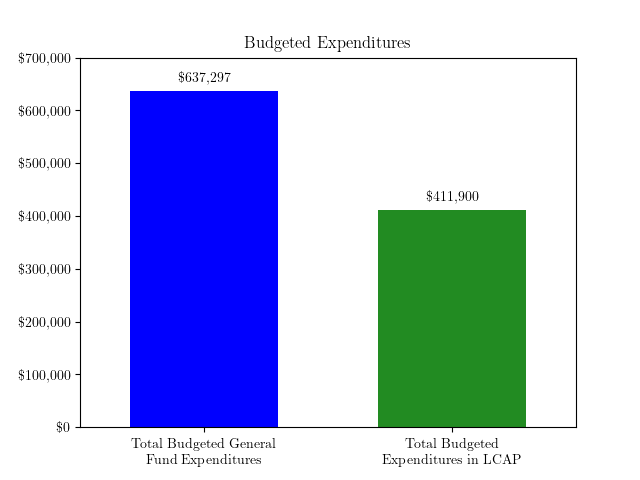
\includegraphics[scale=0.8]{expend}
\caption*{This chart provides a quick summary of how much Sherman Thomas STEM Academy plans to spend for 2019--20. It shows how much of the total is tied to planned actions and services in the LCAP.}
\end{figure}

Sherman Thomas STEM Academy plans to spend \dollar{637297.00} for the 2019--20 school year. Of that amount, \dollar{411900.00} is tied to actions/services in the LCAP and \dollar{225397.00} is not included in the LCAP. The budgeted expenditures that are not included in the LCAP will be used for the following:
\begin{itemize}[noitemsep]
	\item Salaries (office manager and part time: yard duty, director, district secretary, maintenance, janitorial)
	\item Facility Costs (electricity, phones, repair)
	\item Contracts (legal fees, SIS, oversight fees)
	\item Classroom and Office Supplies
\end{itemize}

\subsection{Increased or Improved Services for High Needs Students in 2019--20}
In 2019--20, Sherman Thomas STEM Academy is projecting it will receive \dollar{54102.00} based on the enrollment of foster youth, English learner, and low-income students. Sherman Thomas STEM Academy must demonstrate the planned actions and services will increase or improve services for high needs students compared to the services all students receive in proportion to the increased funding it receives for high needs students. In the LCAP, Sherman Thomas STEM Academy plans to spend \dollar{59918.00} on actions to meet this requirement.

\begin{figure}[h!btp]
\centering
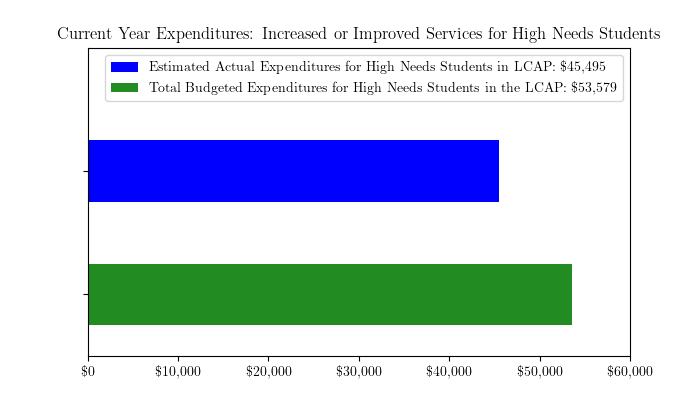
\includegraphics[scale=0.8]{serv}
\caption*{This chart compares what Sherman Thomas STEM Academy budgeted last year in the LCAP for actions and services that contribute to increasing or improving services for high needs students with what  Sherman Thomas STEM Academy estimates it has spent on actions and services that contribute to increasing or improving services for high needs students in the current year.}
\end{figure}

In 2018--19, Sherman Thomas STEM Academy's LCAP budgeted \dollar{53579.00} for planned actions to increase or improve services for high needs students. Sherman Thomas STEM Academy estimates that it will actually spend \dollar{45495.00} for actions to increase or improve services for high needs students in 2018--19. The difference between the budgeted and actual expenditures of \dollar{8084.00} had the following impact on Sherman Thomas STEM Academy's ability to increase or improve services for high needs students:
 
\begin{quotation}
The difference in spending did not impact the actions and services for high needs students. Our field trip costs ended up being much lower than originally anticipated (we budgeted on group discount numbers---not school group), even with us attending three more field trips than originally planned. Also, we no longer pay an EL Coordinator stipend, but rather it is an additional listed job duty on the teacher's contract. Our contract for our reading and math program was also cheaper than originally anticipated. We completed all actions listed in our LCAP and exceeded all goals, with less money being expended.
\end{quotation}

\title{Local Control Accountability Plan and Annual Update (LCAP) Template}
\author{
%\begin{itemize}[label={},noitemsep]
	%\item LEA Name: Sherman Thomas STEM Academy
	%\item Contact Name and Title: Jamie Brock, Principal
	%\item Email and Phone: jabrock\@stcsca.org; 559-871-5490
	%\item LCAP Year: 2019--20
%\end{itemize}
LEA Name: Sherman Thomas STEM Academy\\
Contact Name and Title: Jamie Brock, Principal\\
Email and Phone: jabrock@stcsca.org; 559-871-5490\\
LCAP Year: 2019--20
}
\date{}

\maketitle

\section{2017--20 Plan Summary}
\subsection{The Story}
Describe the students and community and how the LEA serves them.
\begin{quotation}
	We are a new small STEM (Science, Technology, Engineering, and Mathematics) middle school, serving 75 students in grades six, seven, and eight with a college and career emphasis. Our grand opening was August 21, 2017. Our student demographic information is \SI{64}{\percent} Hispanic, \SI{30}{\percent} Caucasian, \SI{3}{\percent} African American, \SI{3}{\percent} Asian, and \SI{50}{\percent} of our students are unduplicated (English Learners, free/reduced lunch, foster/homeless youth).

	One of the things that is exciting about our demographic is that it truly is a cross-section of Madera. Our students do not all live in the same area because attending our schools is not based on a child's address (although preference is given to all students living within Madera Unified School District). Of our current 75 students, we have students who have come from 17 different schools (public, public charter, and private) within Madera. This provides a great opportunity for creating a community celebrating differences.

	Something that makes us unique is that we are the first STEM school in our county. We believe in an integrative instructional model where we apply the principles of the subjects of STEM, Science (hypothesizing and investigating), Technology (improvements that foster ease of a task), Engineering (design process), and Mathematics (identifying problems and persevering to solve them) in all subject areas. Our motto, Dream it, Think it, Do it, is a constant focal point. The lessons are designed to be engaging and interactive with our Fridays, which are specifically set aside for hands on projects, college and career emphasis, field trips, and guest speakers. We are excited to bring these opportunities to the children of our entire community.
\end{quotation}

\subsection{LCAP Highlights}
\begin{quotation}
	{\bf 2017--2020 LCAP Goals:}
	\begin{enumerate}
		\item To prepare students through rigorous and relevant content, to be productive and successful citizens by developing a strong work ethic, and the higher level critical thinking skills needed to solve problems in the 21\st century world.
		\item For all parents to embrace their VOICE (Volunteer, Outings, Inform, Challenge Days, Engage)
		\item To provide a safe, positive, organized setting with clearly defined behavior expectations where effective character education enhances the academic program, while developing habits of professionalism.
	\end{enumerate}
	Being a small school, there is not a lot of revenue, but small class and school size is important to our parents and staff. A key element of our school, that with the exception of salaries and our facility lease, has the largest apportionment of our funds, is our field trip program. We believe it is vital to a child's education to foster higher-level critical thinking skills, and a well-rounded character education program that focuses on professionalism to get students ``in the field.'' In year one (2017--18), all students got to go to 3 college campuses (Reedley College, Fresno State University, and California Polytechnic University San Luis Obispo), 4 community business trips, and 3 enrichment field trips, including Knott's Berry Farm for their Middle School Physics Day and Medieval Times. This current year (2019--19) students visited 4 college campuses (Fresno City, UC Merced, UC Davis, and the California Health Science University), 7 local businesses, and went on 2 enrichment trips. College, and careers to a different extent, seem far away and mysterious to students in this age group in our community. We want kids to see these possibilities as accessible and to understand there are steps they can take, even now, in middle school, to put them on a realistic pathway toward their dreams. We not only wish to open their minds to these possibilities but help build habits they can use on their way through high school and college or higher education training programs. This is a key to our program and is a continued goal for this year. We will be visiting 3 college campuses (Madera Community College Center, Fresno Pacific University, and Stanford University) at least 3 local businesses, and taking all students to a science camp.
\end{quotation}

\subsection{Review of Performance}

\subsubsection{Greatest Progress}
Based on a review of performance on the state indicators and local performance indicators included in the California School Dashboard, progress toward LCAP goals, local self-assessment tools, stakeholder input, or other information, what progress is the LEA most proud of and how does the LEA plan to maintain or build upon that success? This may include identifying any specific examples of how past increases or improvements in services for low-income students, English learners, and foster youth have led to improved performance for these students.
\begin{quotation}	
	We have had a great second year at the Academy. Our year one test scores were the highest in our city, which we are using as a motivator for our 2018--19 testing (which has not yet begun, and therefore we do not have results). We encourage our students to work hard every day---that's what it means to be a Raven. We are proud to have reached all expected measurable outcomes set forth in the previous year's LCAP that we have data on at this point. On local assessments, \SI{75}{\percent} of our students have grown at least one year and/or are at grade level in reading and mathematics, school wide. Over \SI{90}{\percent} of our Stakeholders report being highly satisfied with our school.
\end{quotation}

\subsubsection{Greatest Needs}
Referring to the California School Dashboard, identify any state indicator or local performance indicator for which overall performance was in the ``Red'' or ``Orange'' category or where the LEA received a ``Not Met'' or ``Not Met for Two or More Years'' rating. Additionally, identify any areas that the LEA has determined need significant improvement based on review of local performance indicators or other local indicators. What steps is the LEA planning to take to address these areas with the greatest need for improvement?
\begin{quotation}
	Since 2017--18 was our school's first year of existence, we do not have any ``red'' or ``orange'' performance categories. Last year was our school's first time taking the CAASPP, so our scores are being used as baseline data. This year, 2018--19 will be our first chance to show increase or decline, and therefore will be our first time having ``colors.'' That being said, we do have areas of concern that we as a staff are working to address. While we met our goal of \SI{75}{\percent} of students growing a minimum of one year and/or being at grade level in reading and math, we barely met it (\SI{74.8}{\percent}). We see this as an area for us to work on and are looking for ways to improve. This was a \SI{4.78}{\percent} increase over last year, but we were hoping to see greater growth.
\end{quotation}

\subsubsection{Performance Gaps}
Referring to the California School Dashboard, identify any state indicator for which performance for any student group was two or more performance levels below the ``all student'' performance. What steps is the LEA planning to take to address these performance gaps?
\begin{quotation}
	Since 2017--18 was our first year testing and we do not have data for 2018--19 yet, we don't have any state indicators on the Dashboard. That being said, I do have data broken down by subgroup for the 2017--18 results (we have not yet done our 2018--19 testing). Overall, our school had \SI{74}{\percent} of our students meet/exceed standard in English and \SI{55}{\percent} met/exceeded standard in math. We had several subgroups that performed below this---which I would see as a gap to be addressed. Our Hispanic students were \SI{5}{\percent} below in English and \SI{6}{\percent} below in Math. Our socio-economically disadvantaged students were \SI{7}{\percent} below in English and \SI{22}{\percent} below in math (this is the biggest and most concerning gap). Our boys were also \SI{4}{\percent} below in English and \SI{6}{\percent} below in Math. Our highest performing subgroup in Math was our white students, with \SI{68}{\percent} meeting/exceeding standard and our girls, with \SI{64}{\percent}. Our highest performing sub-group in English were our RFEP students, with \SI{91}{\percent} meeting/exceeding standard. Most of our sub-groups were within \SI{10}{\percent} of our overall score, which I don't consider to be a significant performance gap.
\end{quotation}

\subsection{Comprehensive Support and Improvement}
An LEA with a school or schools identified for comprehensive support and improvement (CSI) under the Every Student Succeeds Act must respond to the following prompts.

\subsubsection{Schools Identified}
Identify the schools within the LEA that have been identified for CSI.
\begin{quote}
	No schools within the LEA have been identified for CSI
\end{quote}

\subsubsection{Support for Identified Schools}
Describe how the LEA supported the identified schools in developing CSI plans that included a school-level needs assessment, evidence-based interventions, and the identification of any resource inequities to be addressed through the implementation of the CSI plan.
\begin{quote}
	NA
\end{quote}

\subsubsection{Support for Identified Schools}
Describe how the LEA will monitor and evaluate the implementation and effectiveness of the CSI plan to support student and school improvement.
\begin{quote}
	NA
\end{quote}

\section{Annual Update}
{\bf LCAP Year Reviewed: 2018--19}\newline
Complete a copy of the following table for each of the LEA's goals from the prior year LCAP. Duplicate the table as needed.

\Goal %1
	{To prepare students, through rigorous and relevant content, to be productive and successful citizens by developing a strong work ethic and the higher-level critical thinking skills needed to solve problems in the 21\st century world.}
	{1, 2, 4, 7, 8}
	{}

\begin{outcomes}
	\outcome
		{Teacher Certification: \SI{100}{\percent} appropriately assigned and fully credentialed.}
		{\SI{100}{\percent} appropriately assigned and fully credentialed.}
	\outcome
		{Instructional Materials Quarterly Self Audit: ALL students will have access to standards-aligned instructional materials.}
		{All students had access to standards-aligned instructional materials.}
	\outcome
		{CAASPP Results: \SI{98}{\percent} Participation Rate. To be in the ``increased level'' for mean distance from Level 3 in ELA and Math.}
		{Pending test results (students test in May)}
	\outcome
		{CELDT Results: \SI{70}{\percent} of EL pupils will grow one level or be re\-designated.}
		{Pending test results (students test at end of April)}
	\outcome
		{Renaissance Results: \SI{75}{\percent} of students will be at grade level in ELA and Math and/or grow a minimum of 1 year.}
		{\SI{74.8}{\percent} of students were at grade level in ELA and Math and/or grew a minimum of 1 year.}
\end{outcomes}

\subsubsection{Actions/Services}
Duplicate the Actions/Services from the prior year LCAP and complete a copy of the following table for each. Duplicate the table as needed.
\actionupdate
	{Teacher contracts (including principal/teacher combo role) -- salary + benefits. (Only \SI{90.2}{\percent} of 6\th grade teacher, as the remaining \SI{9.8}{\percent} is in a different action for intervention).}
	{Teacher contracts (including principal/teacher combo role) -- salary + benefits. (Only \SI{90.2}{\percent} of 6\th grade teacher, as the remaining \SI{9.8}{\percent} is in a different action for intervention).}
	{228701}
	{242423}

\actionupdate
	{Weekly PLC meetings; outside professional development}
	{Weekly PLC meetings; outside professional development}
	{10000}
	{8115.22}

\actionupdate
	{Technology infrastructure and support to ensure internet capability on all devices.}
	{Technology infrastructure and support to ensure internet capability on all devices.}
	{15000}
	{11215}

\actionupdate
	{Intervention Program (\SI{9.8}{\percent}) of 6\th grade teacher's salary)}
	{Intervention Program (\SI{9.8}{\percent}) of 6\th grade teacher's salary)}
	{7292}
	{8686}

\actionupdate
	{EL Coordinator}
	{EL Coordinator}
	{2000}
	{\dollar{0} (embedded in salary)}

\actionupdate
	{Renaissance Program and End of Year Field Trip}
	{Renaissance Program and End of Year Field Trip}
	{8000}
	{5739}

\actionupdate
	{Classified Employee working with students as a classroom aid in the morning.}
	{Classified Employee working with students as a classroom aid in the morning.}
	{5300}
	{5300}

\subsubsection{Analysis}
Complete a copy of the following table for each of the LEA's goals from the prior year LCAP. Duplicate the table as needed. Use actual annual measurable outcome data, including performance data from the LCFF Evaluation Rubrics, as applicable.

Describe the overall implementation of the actions/services to achieve the articulated goal.
\begin{quotation}
	All stated actions were implemented to achieve the articulated goal.
	\begin{actionanalysis}
	\item \SI{100}{\percent} of teachers were appropriately assigned and fully credentialed.
	\item Teaching staff met at least weekly both formally and ad-hoc to discuss planning, student achievement, teaching strategies, classroom management, and other areas of strengths and weaknesses as they arose. Our entire team attended the International Literacy Association Conference and our principal attended the Charter School Development Leadership Update Conference.
	\item All technology has been purchased and the infrastructure is in place to support all students being able to be on a device with internet at one time. Our contract for tech support, through Madera County Superintendent of Schools allows us to ensure that all updates are done in a timely manner---for both testing purposes as well as student safety (filtration system).
	\item We implemented and ran an intervention program the last 45 minutes of each day Monday -- Thursday that focused on a variety of topics based on highest need as observed by each classroom teacher.
	\item Our EL Coordinator attended all trainings, monitored progress of EL students, and administered the ELPAC test.
	\item We purchased the Renaissance Program to monitor and track student achievement as measured by reading and math levels and administered the tests throughout the year to monitor growth. We will be taking students who have met the goal on an end of year reward trip.
	\item One of our classified employees works with students as a classroom aid each morning, assisting students with questions and comprehension in science.
	\end{actionanalysis}
\end{quotation}

Describe the overall effectiveness of the actions/services to achieve the articulated goal as measured by the LEA.
\begin{quotation}
	Through the above mentioned actions we believe that we were able to achieve our expected annual measurable outcomes as we continue to strive to fully reach this goal. There is still room for growth, but we have met our year one and two outcomes. There are still some areas that we do not know the results of yet, but we have achieved all outcomes that we have information for at this time. We believe that by continuing to reach for and achieve these specific measurable outcomes, that we will reach our goal of preparing students for the 21\st century world.
\end{quotation}

Explain material differences between Budgeted Expenditures and Estimated Actual Expenditures.
\begin{quotation}
	We are still calculating final expenditures, but at this time, there do not appear to be any material differences between Budget Expenditures and Estimated Actual Expenditures. One area that changed this year is the EL Stipend. In 2017--18, it was a stipend and that was the plan at the beginning of this year. Instead, the job duty was added to the teacher's contract and she was given a raise. Our estimated actuals, for this goal, are approximately \dollar{5000} higher than budgeted, which is mainly due to a higher than anticipated cost in employee benefits. Projections were based off of approximately \SI{30}{\percent} of an employee's salary, when in reality it was closer to \SI{37}{\percent} due to rising costs.
\end{quotation}

Describe any changes made to this goal, expected outcomes, metrics, or actions and services to achieve this goal as a result of this analysis and analysis of the LCFF Evaluation Rubrics, as applicable. Identify where those changes can be found in the LCAP.
\begin{quotation}
	We have not made any changes to this goal and will continue to work hard to achieve it. The only change that has been made for 2019--20, is that the EL Coordinator has a \dollar{0} cost because it is embedded into the teacher's salary.
\end{quotation}

\Goal
	{For all parents to embrace their VOICE (Volunteer, Outings, Inform, Challenge Days, Engage) at STA}
	{3}
	{}

\begin{outcomes}
	\outcome
	{\SI{65}{\percent} Parent Participation in at least one of our evening events}
	{\SI{89}{\percent} Parent Participation in at least one of our evening events}
	\outcome
	{\SI{20}{\percent} Parent Participation in at least one challenge day and/or field trip}
	{\SI{36}{\percent} Parent Participation in at least one challenge day and/or field trip}
	\outcome
	{\SI{30}{\percent} Parent Participation in at least one STAff chat}
	{\SI{44}{\percent} Parent Participation in at least one STAff chat}
	\outcome
	{\SI{45}{\percent} Parent Participation in one or more parent-teacher conferences during the year}
	{\SI{87}{\percent} Parent Participation in one or more parent-teacher conferences during the year}
\end{outcomes}

\subsubsection{Actions/Services}
Duplicate the Actions/Services from the prior year LCAP and complete a copy of the following table for each. Duplicate the table as needed.
\actionupdate
	{Parent communication (Promote a culture providing ways for parents to be involved)}
	{Parent Communication (Promoted a culture providing ways for parents to be involved)}
	{\dollar{0} (embedded in salaries)}
	{\dollar{0} (embedded in salaries)}

\actionupdate
	{Parent Communication (email, newsletters, Facebook, etc.)}
	{Parent Communication (email, newsletters, Facebook, Remind, etc.)}
	{\dollar{0} (embedded in salaries)}
	{\dollar{0} (embedded in salaries)}

\subsubsection{Analysis}
Complete a copy of the following table for each of the LEA's goals from the prior year LCAP. Duplicate the table as needed. Use actual annual measurable outcome data, including performance data from the LCFF Evaluation Rubrics, as applicable.

Describe the overall implementation of the actions/services to achieve the articulated goal.
\begin{quotation}
	All actions were implemented to achieve this articulated goal.
	\begin{actionanalysis}
	\item Parents were informed, on a regular basis, of ways that they could be involved at the school. Almost half attended a monthly STAff chat, to provide input on the running of the school and LCAP. \SI{89}{\percent} participated in an evening event with their families. \SI{36}{\percent} helped with a field trip and/or challenge day. Multiple avenues for active parent involvement were regularly presented and parents participated.
	\item Parents were communicated with frequently. At the end of every week the principal sent an email highlighting events of the week, which included pictures, to help with discussions in the home. The principal also posted multiple pictures and videos on Facebook (weekly). At the beginning of each week the principal emailed all parents important information for the week, including meetings, practices, field trips, and ways to be involved. A quarterly newsletter was given out at each family night. All teachers notified parents on a weekly basis of all homework for the week. Lastly, parents received a packet every Monday with a grade check and all work from the previous week (including teacher feedback). In our 2018--19 parent survey, the most common thing that was mentioned that we do well is communication. Parents feel informed and they like it.
	\end{actionanalysis}
\end{quotation}

Describe the overall effectiveness of the actions/services to achieve the articulated goal as measured by the LEA.
\begin{quotation}
	Our goal was for all parents to embrace their VOICE at STA and I believe we have achieved this goal. For the second year in a row, we exceeded our expected measurable outcomes, in each area. Our parents have repeatedly voiced how much they love our school and their sadness that it is only a 3 year program. I feel confident they have embraced their VOICE at STA through the culture we have created from frequent communication.
\end{quotation}

Explain material differences between Budgeted Expenditures and Estimated Actual Expenditures.
\begin{quotation}
	There are no material differences between Budgeted Expenditures and Estimated Actual Expenditures because there are no expenditures. The amount budgeted is \dollar{0}---it is embedded within the teacher salaries.
\end{quotation}

Describe any changes made to this goal, expected outcomes, metrics, or actions and services to achieve this goal as a result of this analysis and analysis of the LCFF Evaluation Rubrics, as applicable. Identify where those changes can be found in the LCAP.
\begin{quotation}
	The only change we are making is the addition of usage of the app ``Remind.'' Some parents have voiced an interest in using a communication app, as a way of sending text alerts. We decided on Remind because most of our graduating 8\th graders will be going to schools within our authorizer's district and the high schools there use Remind. Other than that, we are making no changes. It is our goal to continue to foster an environment where parents feel that they are an integral part of our program and that they have a VOICE at STA.
\end{quotation}

\Goal
	{To provide a safe, positive, organized setting with clearly defined behavior expectations where effective character education enhances the academic program, while developing habits of professionalism.}
	{1, 5, 6, 7}
	{}

\begin{outcomes}
	\outcome
	{Facility Evaluations: \SI{100}{\percent} of monthly evaluations will receive a ``good rating''}
	{\SI{100}{\percent} of monthly evaluations received a good rating}
	\outcome
	{Attendance Rate: \SI{93}{\percent}}
	{\SI{99}{\percent}}
	\outcome
	{Chronic Absenteeism: Less than \SI{3}{\percent}}
	{\SI{0}{\percent}}
	\outcome
	{Middle School Dropout Rate: Less than \SI{1.5}{\percent}}
	{\SI{0}{\percent}}
	\outcome
	{Pupil Suspension Rate: Less than \SI{6}{\percent}}
	{\SI{4}{\percent}}
	\outcome
	{Pupil Expulsion Rate: Less than \SI{1.5}{\percent}}
	{\SI{0}{\percent}}
	\outcome
	{School Climate Survey to all Stakeholders: \SI{80}{\percent} Satisfaction}
	{\SI{94}{\percent} Overall satisfaction on school climate survey}
	\outcome
	{Diverse Enrichment Field Trips and Opportunities: 3 colleges, 3 community businesses, and 1 enrichment standards aligned field trip}
	{4 colleges, 7 community businesses, and 1 enrichment standards aligned field trip}
\end{outcomes}

\subsubsection{Actions/Services}
Duplicate the Actions/Services from the prior year LCAP and complete a copy of the following table for each. Duplicate the table as needed.

\actionupdate
	{Facility Lease}
	{Facility Lease}
	{72000}
	{72000}

\actionupdate
	{Student Study Team}
	{Student Study Team}
	{0}
	{0}

\actionupdate
	{School Climate Survey}
	{School Climate Survey}
	{0}
	{0}

\actionupdate
	{Field Trip Program: Costs to cover transportation, food, and admission for all students}
	{Field Trip Program: Cost covered transportation, food, and admission for all students}
	{25000}
	{17655}

\subsubsection{Analysis}
Complete a copy of the following table for each of the LEA's goals from the prior year LCAP. Duplicate the table as needed. Use actual annual measurable outcome data, including performance data from the LCFF Evaluation Rubrics, as applicable.

Describe the overall implementation of the actions/services to achieve the articulated goal.
\begin{quotation}
	All actions were implemented to achieve the articulated goal.
	\begin{actionanalysis}
	\item We have secured a long-term facility lease in a building that is perfectly suited and designed to meet our needs. Through the Walton Family Foundation Grant, we were able to fund landscaping and a recreational area for the students, which has fostered character education. We have taught our students what it means to take care of their belongings and they are doing a great job.
	\item Our Student Study Team has met with students for academic, behavior, and attendance issues to work on strategies for improvement in the area of concern.
	\item We conducted a school climate survey with our parents as well as students. \SI{94}{\percent} of those surveyed reported being satisfied with our overall program. \SI{94}{\percent} of our parents reported that their child feels safe at school.
	\item We implemented and fully ran our field trip program. All students went to 4 colleges, 7 local businesses, and participated in 2 enrichment field trips for a total of 13 field trips.
	\end{actionanalysis}
\end{quotation}

Describe the overall effectiveness of the actions/services to achieve the articulated goal as measured by the LEA.
\begin{quotation}
	We exceeded every expected annual measurable outcome set for the 2018--19 school year. All field trips were designed to enhance character education and/or develop habits of professionalism. We believe providing these opportunities brings meaning to the classroom and context. Having adults share the importance of education and constantly showing students the ``end game'' helps with motivation. We have an excellent attendance rate, minimal suspension, and very few behavior issues. We have worked hard to create a culture of excellence where students feel safe and strive to do their best.
\end{quotation}

Explain material differences between Budgeted Expenditures and Estimated Actual Expenditures.
\begin{quotation}
	We are still calculating final expenditures, but at this time, there do not appear to be any material differences between Budget Expenditures and Estimated Actual Expenditures.
\end{quotation}

Describe any changes made to this goal, expected outcomes, metrics, or actions and services to achieve this goal as a result of this analysis and analysis of the LCFF Evaluation Rubrics, as applicable. Identify where those changes can be found in the LCAP.
\begin{quotation}
	No changes were made to this goal, expected outcomes, metrics, or actions and services.
\end{quotation}

\section{Stakeholder Engagement}
{\bf LCAP Year: 2019--20}

\subsection{Involvement Process for LCAP and Annual Update}
How, when, and with whom did the LEA consult as part of the planning process for this LCAP/Annual Review and Analysis?
\begin{quotation}
	Every month, our school has something that we call STAff chat (STA is our school abbreviation---so it is a play on our initials and the word staff).  The entire staff has attended at least one of these chats as well as almost half of our parents. The principal/8\th grade teacher and 6\th grade teacher have been at all and ran them. At these monthly meetings, we always go over things that we have done as well as any upcoming events. We end each one with a time of discussion---asking parents for input regarding things that we are doing well and areas for improvement. We also specifically address budgetary issues and discuss possible ideas regarding changes for the future. Our parents have been educated on the LCAP and its purpose and given opportunities to provide feedback.

	Our teachers are not part of a bargaining unit, but all staff (classified and certified) were consulted regarding the LCAP, through STAff chats as well as staff meetings.

	In addition to monthly STAff chats, we also have monthly board meetings, where community stakeholders were given time to provide input regarding STA. They were also given updates on items discussed in the 2018--19 LCAP budget and given opportunity for feedback regarding decisions being made.

	We also have a student council who meets weekly with the principal. They plan upcoming events and also provide meaningful feedback, sharing what they like and possible areas for improvement.

	The site principal also consulted, regularly, with the Sherman Thomas Charter Schools fiscal analyst to ensure that expenditures were within the budget and to confirm budgetary numbers for the 2019--20 school year.
\end{quotation}

\subsection{Impact on LCAP and Annual Update}
How did these consultations impact the LCAP for the upcoming year?
\begin{quotation}
	As we anticipated, we have learned, through monthly STAff chats as well as a parent and student surveys, that our field trip program is very important to our parents. They are extremely appreciative of the opportunities afforded to ALL students at the Academy and the fact that everyone gets to attend for free without any fundraising. This has proven to be very popular amongst parents and students. We all see the value that this hands on experience gives to students in their education and will continue to have our field trip budget be one of the largest areas of allotted funds.

	Through these consultations, we found that there were very few areas that stakeholders wished to be changed. The one area that some parents and students did wish we had was sports. We do not run an athletic program. When we explained to parents why we do not participate in the MULES league, they understood. There is also a great opportunity for our 7\th and 8\th grade students to compete for the MUSD middle school whose boundary they reside in, which many of our students have taken advantage of. We have had students compete at Thomas Jefferson, Martin Luther King, and Desmond Middle School in football, volleyball, golf, cross country, wrestling, basketball, track and field, soccer, and swimming.

	We are running a program that fosters collaboration and habits of professionalism. Our parents feel that they are integral in their child's education and have found their VOICE. Our students feel safe, accepted, and want to be at school. It appears that all three goals we set are areas that our stakeholders still value and we will continue to work towards making them become an even stronger reality.
\end{quotation}

\section{Goals, Actions, \& Services}
Strategic Planning Details and Accountability\newline
Complete a copy of the following table for each of the LEA's goals. Duplicate the table as needed.

\Goal[Unchanged]
	{To prepare students, through rigorous and relevant content, to be productive and successful citizens by developing a strong work ethic and the higher-level critical thinking skills needed to solve problems in the 21\st century world.}
	{1, 2, 4, 7, 8}
	{}
	{Fully credentialed teachers with EL certification, \SI{100}{\percent} of students with access to state board adopted content and performance standards aligned lessons including EL students and individuals with exceptional needs, and growth of students in ELA and Mathematics.}

\begin{expoutcomes}
	\expoutcome
	{Teacher Certification}
	{Establishing in 2017--18}
	{\SI{100}{\percent} appropriately assigned and fully credentialed.}
	{\SI{100}{\percent} appropriately assigned and fully credentialed.}
	{\SI{100}{\percent} appropriately assigned and fully credentialed.}
	\expoutcome
	{Instructional Materials Quarterly Self-Audit}
	{Establishing in 2017-18}
	{ALL students will have access to standards-aligned instructional materials.}
	{ALL students will have access to standards-aligned instructional materials.}
	{ALL students will have access to standards-aligned instructional materials.}
	\expoutcome
	{CAASPP Results}
	{Establishing in 2017-18}
	{\SI{97}{\percent} Participation Rate. Establish baseline data.}
	{\SI{98}{\percent} Participation Rate. To be in the ``increased level'' for mean distance from Level 3 in ELA and Math.}
	{\SI{98}{\percent} Participation Rate. To be in the ``maintained level'' for mean distance from Level 3 in ELA and Math.}
	\expoutcome
	{ELPAC Results}
	{Establishing in 2017-18}
	{\SI{67}{\percent} of EL pupils will grow one level or be re-designated.}
	{\SI{70}{\percent} of EL pupils will grow one level or be re-designated.}
	{\SI{75}{\percent} of EL pupils will grow one level or be re-designated.}
	\expoutcome
	{Renaissance and IXL Results}
	{Establishing in 2017-18}
	{\SI{70}{\percent} of students will be at grade level in ELA and Math and/or grow a minimum of 1 year.}
	{\SI{75}{\percent} of students will be at grade level in ELA and Math and/or grow a minimum of 1 year.}
	{\SI{80}{\percent} of students will be at grade level in ELA and Math and/or grow a minimum of 1 year.}

\end{expoutcomes}

\begin{planactions}[Complete a copy of the following table for each of the LEA's Actions/Services. Duplicate the table, including Budgeted Expenditures, as needed.]
	\planaction
	{Ensure \SI{100}{\percent} of teaching staff will be fully credentialed and highly qualified to teach all subjects and have EL certification.}
	\planaction@scope
	{All}{All Schools}
	\planaction@action
	{New}{Modified}{Modified}
	{Teacher Contracts (including principal/teacher combo role) -- salary + benefits. Only \SI{90.2}{\percent} of 6\th grade teacher as the remaining \SI{9.8}{\percent} is in a different action for intervention.}
	{Teacher Contracts (including principal/teacher combo role) -- salary + benefits. Only \SI{90.2}{\percent} of 6\th grade teacher as the remaining \SI{9.8}{\percent} is in a different action for intervention.}
	{Teacher Contracts (including principal/teacher combo role) -- salary + benefits. Only \SI{90.2}{\percent} of 6\th grade teacher as the remaining \SI{9.8}{\percent} is in a different action for intervention.}
	\planaction@budget
	{199932}{228701}{254982}
	{LCFF Base}{LCFF Base}{LCFF Base}
	{\num{1000} and \num{3000} Certified Salaries and Benefits}
	{\num{1000} and \num{3000} Certified Salaries and Benefits}
	{\num{1000} and \num{3000} Certified Salaries and Benefits}

	\planaction
	{Provide training to staff to ensure that ALL students have access to standards-aligned instructional materials that are addressing all state board approved academic content and performance standards for grades 6 -- 8. This will be through weekly PLC meetings as well as outside Professional Development, based on teacher input and administrative approval.}
	\planaction@scope
	{All}{All Schools}
	\planaction@action
	{New}{Modified}{Modified}
	{Weekly PLC meetings; outside professional development}
	{Weekly PLC meetings; outside professional development}
	{Weekly PLC meetings; outside professional development}
	\planaction@budget
	{7000}{10000}{10000}
	{LCFF Base}{Supplemental and Concentration}{LCFF Base}
	{\num{5000} Services and Other Operating Expenses}
	{\num{5000} Services and Other Operating Expenses}
	{\num{5000} Services and Other Operating Expenses}
	
	\planaction
	{Students will participate in ALL statewide assessments and show growth in all areas. Ensure that all infrastructure, in terms of technology, is in place for assessments.}
	\planaction@scope
	{All}{All Schools}
	\planaction@action
	{New}{Unchanged}{Unchanged}
	{Technology infrastructure and support to ensure internet capability on all devices.}
	{Technology infrastructure and support to ensure internet capability on all devices.}
	{Technology infrastructure and support to ensure internet capability on all devices.}
	\planaction@budget
	{15000}{15000}{15000}
	{LCFF Base}{LCFF Base}{LCFF Base}
	{\num{4000} and \num{5000} Books and Supplies, Services and Other Operating Expenses}
	{\num{4000} and \num{5000} Books and Supplies, Services and Other Operating Expenses}
	{\num{4000} and \num{5000} Books and Supplies, Services and Other Operating Expenses}

	\planaction*
	{Create an intervention program that targets specific skills and specific students in two to three week rotations.}
	\planaction@scope
	{English Learners, Foster Youth, and Low Income}
	{LEA-wide}
	{All Schools}
	\planaction@action
	{New}{Modified}{Modified}
	{Intervention Program (\SI{9.8}{\percent} of 6\th grade teacher's salary and benefits)}
	{Intervention Program (\SI{9.8}{\percent} of 6\th grade teacher's salary and benefits)}
	{Intervention Program (\SI{9.8}{\percent} of 6\th grade teacher's salary and benefits)}
	\planaction@budget
	{6468}{7899}{8918}
	{Supplemental and Concentration}
	{Supplemental and Concentration}
	{Supplemental and Concentration}
	{\num{1000} and \num{3000} Certificated Salaries and Benefits}
	{\num{1000} and \num{3000} Certificated Salaries and Benefits}
	{\num{1000} and \num{3000} Certificated Salaries and Benefits}

	\planaction*
	{Ensure that all EL students are making progress towards their goals and that all assessments and parent communication happens in a timely manner.}
	\planaction@scope
	{English Learners}{Limited to Unduplicated Students}{All Schools}
	\planaction@action
	{New}{Unchanged}{Unchanged}
	{EL Coordinator}{EL Coordinator}{EL Coordinator}
	\planaction@budget
	{2000}{2000}{\dollar{0} (embedded in teacher salary)}
	{Supplemental and Concentration}
	{Supplemental and Concentration}
	{Supplemental and Concentration}
	{\num{1000} Certificated Salaries}
	{\num{1000} Certificated Salaries}
	{NA}

	\planaction*
	{Purchase Renaissance Learning for English and IXL for all subjects, to monitor growth of students in English and Mathematics. For all students who achieve their four-pronged individualized goal (AR points earned, reading level---grade level up and/or growth (using 2 measures---Renaissance and IXL), and math level---grade level up and/or growth) take an end of year reward trip.}
	\planaction@scope
	{English Learners, Foster Youth, and/or Low Income}
	{LEA-wide}
	{All Schools}
	\planaction@action
	{New}{Modified}{Modified}
	{Renaissance Program and end of year reward trip}
	{Renaissance Program and end of year reward trip}
	{Renaissance and IXL Program and end of year reward trip}
	\planaction@budget
	{7000}{8000}{8000}
	{LCFF Base}{Supplemental and Concentration}{Supplemental and Concentration}
	{\num{5000} Services and Other Operating Expenses}
	{\num{5000} Services and Other Operating Expenses}
	{\num{5000} Services and Other Operating Expenses}

	\planaction*
	{A full-time classified employee will work directly with students during the morning, assisting those struggling with grade level material (with a special focus on English Learners and students with exceptional needs). These duties will be approximately \SI{20}{\percent} of their duty day.}
	\planaction@scope
	{English Learners, Foster Youth, Low Income}{LEA-wide}{All Schools}
	\planaction@action
	{New}{Modified}{Modified}
	{Classified Employee working with students as a classroom aid in the morning}
	{Classified Employee working with students as a classroom aid in the morning}
	{Classified Employee working with students as a classroom aid in the morning}
	\planaction@budget
	{4800}{5300}{6000}
	{Supplemental and Concentration}
	{Supplemental and Concentration}
	{Supplemental and Concentration}
	{\num{2000} Classified Salary}
	{\num{2000} Classified Salary}
	{\num{2000} Classified Salary}
\end{planactions}

\Goal[Unchanged]
	{For all parents to embrace their VOICE (Volunteer, Outings, Inform, Challenge Days, Engage) at STA.}
	{3}
	{}
	{Parent participation in our challenge days (hands on projects with the kids), field trips, monthly STAff chats, quarterly family nights, and parent-teacher conferences.}

\begin{expoutcomes}
	\expoutcome
	{Sign-in Sheets}
	{Establishing in 2017--18}
	{\SI{60}{\percent} parent participation in at least one of our evening events.}
	{\SI{65}{\percent} parent participation in at least one of our evening events.}
	{\SI{70}{\percent} parent participation in at least one of our evening events.}
	\expoutcome
	{Sign-in Sheets}
	{Establishing in 2017--18}
	{\SI{15}{\percent} parent participation in at least one challenge day and/or field trip.}
	{\SI{20}{\percent} parent participation in at least one challenge day and/or field trip.}
	{\SI{25}{\percent} parent participation in at least one challenge day and/or field trip.}
	\expoutcome
	{Sign-in Sheets}
	{Establishing in 2017--18}
	{\SI{25}{\percent} parent participation in at least one STAff chat.}
	{\SI{30}{\percent} parent participation in at least one STAff chat.}
	{\SI{35}{\percent} parent participation in at least one STAff chat.}
	\expoutcome
	{Sign-in Sheets and Call Logs}
	{Establishing in 2017--18}
	{\SI{40}{\percent} parent participation in one or more parent-teacher conferences during the year.}
	{\SI{45}{\percent} parent participation in one or more parent-teacher conferences during the year.}
	{\SI{50}{\percent} parent participation in one or more parent-teacher conferences during the year.}
\end{expoutcomes}

\begin{planactions}[Complete a copy of the following table for each of the LEA's Actions/Services. Duplicate the table, including Budgeted Expenditures, as needed.]
	\planaction
	{Promote a culture of volunteerism among parents by providing a variety of ways that they can be involved (i.e. field trips, Friday challenge days, quarterly family nights, monthly STAff chats, and general classroom volunteer work). Parents are the primary educators of children---we want to come alongside them and partner with them to ensure the success of all students.}
	\planaction@scope
	{All}{All Schools}
	\planaction@action
	{New}{Unchanged}{Unchanged}
	{Parent Communication}
	{Parent Communication}
	{Parent Communication}
	\planaction@budget
	{\dollar{0} (embedded in salaries)}
	{\dollar{0} (embedded in salaries)}
	{\dollar{0} (embedded in salaries)}
	{NA}{NA}{NA}{NA}{NA}{NA}

	\planaction
	{Regularly communicate all opportunities for parent engagement through our website, Facebook page, email, Remind app, and newsletter.}
	\planaction@scope
	{All}{All Schools}
	\planaction@action
	{New}{Unchanged}{Unchanged}
	{Parent Communication}
	{Parent Communication}
	{Parent Communication}
	\planaction@budget
	{\dollar{0} (embedded in salaries)}
	{\dollar{0} (embedded in salaries)}
	{\dollar{0} (embedded in salaries)}
	{NA}{NA}{NA}{NA}{NA}{NA}
\end{planactions}

\Goal[Unchanged]
	{To provide a safe, positive, organized setting with clearly defined behavior expectations where effective character education enhances the academic program, while developing habits of professionalism.}
	{1, 5, 6, 7}
	{}
	{Facility with a space that functions for learning objectives, clearly defined behavior expectations laid out in parent/student handbook and discussed with parents and students, student study team for academic, attendance, and behavior issues, and engaging class activities and field trips that promote attendance, behavior, and a more competent 21\st century work force.}

\begin{expoutcomes}
	\expoutcome
	{Facility Lease with monthly ``good'' evaluations}
	{Establishing in 2017--18}
	{\SI{100}{\percent} of monthly evaluations will receive a ``good'' rating.}
	{\SI{100}{\percent} of monthly evaluations will receive a ``good'' rating.}
	{\SI{100}{\percent} of monthly evaluations will receive a ``good'' rating.}
	\expoutcome
	{Attendance Rate}
	{Establishing in 2017--18}
	{\SI{91}{\percent}}
	{\SI{93}{\percent}}
	{\SI{95}{\percent}}
	\expoutcome
	{Chronic Absenteeism}
	{Establishing in 2017--18}
	{Less than \SI{4.5}{\percent}}
	{Less than \SI{3}{\percent}}
	{Less than \SI{3}{\percent}}
	\expoutcome
	{Middle School Dropout Rate}
	{Establishing in 2017--18}
	{Less than \SI{1.5}{\percent}}
	{Less than \SI{1.5}{\percent}}
	{Less than \SI{1.5}{\percent}}
	\expoutcome
	{Pupil Suspension Rate}
	{Establishing in 2017--18}
	{Less than \SI{9}{\percent}}
	{Less than \SI{6}{\percent}}
	{Less than \SI{3}{\percent}}
	\expoutcome
	{Pupil expulsion rate}
	{Establishing in 2017--18}
	{Less than \SI{1.5}{\percent}}
	{Less than \SI{1.5}{\percent}}
	{Less than \SI{1.5}{\percent}}
	\expoutcome
	{School Climate Survey to all Stakeholders}
	{Establishing in 2017--18}
	{\SI{75}{\percent} Satisfaction}
	{\SI{80}{\percent} Satisfaction}
	{\SI{85}{\percent} Satisfaction}
	\expoutcome
	{Diverse Enrichment field trips and opportunities}
	{Establishing in 2017--18}
	{3 colleges, 3 community businesses, and 1 enrichment standards-aligned field trip.}
	{3 colleges, 3 community businesses, and 1 enrichment standards-aligned field trip.}
	{3 colleges, 3 community businesses, and 1 enrichment standards-aligned field trip.}
\end{expoutcomes}

\begin{planactions}[Complete a copy of the following table for each of the LEA's Actions/Services. Duplicate the table, including Budgeted Expenditures, as needed.]
	\planaction
	{Secure a lease for a facility with a large space to accommodate 75 students at one time, with regular maintenance.}
	\planaction@scope
	{All}{All Schools}
	\planaction@action
	{New}{Unchanged}{Unchanged}
	{Facility Lease}
	{Facility Lease}
	{Facility Lease}
	\planaction@budget
	{72000}{72000}{72000}
	{LCFF Base}{LCFF Base}{LCFF Base}
	{\num{5000} Services and Other Operating Expenses}
	{\num{5000} Services and Other Operating Expenses}
	{\num{5000} Services and Other Operating Expenses}

	\planaction
	{All teachers and principal participate in the student study team that meets to discuss students that are deemed ``at risk,'' which could include issues with academics, attendance, and/or behavior, to address issues before they become a significant problem.}
	\planaction@scope
	{All}{All Schools}
	\planaction@action
	{New}{Unchanged}{Unchanged}
	{Student Study Team}
	{Student Study Team}
	{Student Study Team}
	\planaction@budget
	{\dollar{0} (embedded in salaries)}
	{\dollar{0} (embedded in salaries)}
	{\dollar{0} (embedded in salaries)}
	{NA}{NA}{NA}{NA}{NA}{NA}

	\planaction
	{Give a school climate survey to determine school culture/climate satisfaction to students, parents, and other meaningful stakeholders.}
	\planaction@scope
	{All}{All Schools}
	\planaction@action
	{New}{Unchanged}{Unchanged}
	{School climate survey}
	{School climate survey}
	{School climate survey}
	\planaction@budget
	{\dollar{0} (embedded in salaries and technology costs)}
	{\dollar{0} (embedded in salaries and technology costs)}
	{\dollar{0} (embedded in salaries and technology costs)}
	{NA}{NA}{NA}{NA}{NA}{NA}
	
	\planaction*
	{ALL students will have access to our field trip and enrichment program that will include a minimum of 3 college campus visits, 3 community businesses, and 1 standards aligned enrichment field trip for no charge, ensuring equal access to all.}
	\planaction@scope
	{English Learners, Foster Youth, and/or Low Income}
	{LEA-wide}
	{All Schools}
	\planaction@action
	{New}{Modified}{Modified}
	{Field Trip program; costs to cover transportation, food, and admission for all students}
	{Field Trip program; costs to cover transportation, food, and admission for all students}
	{Field Trip program; costs to cover transportation, food, and admission for all students}
	\planaction@budget
	{21000}{25000}{37000}
	{LCFF Base}
	{Supplemental and concentration}
	{Supplemental and concentration}
	{\num{5000} Services and Other Operating Expenses} 
	{\num{5000} Services and Other Operating Expenses} 
	{\num{5000} Services and Other Operating Expenses} 
\end{planactions}

\section{Demonstration of Increased or Improved Services for Unduplicated Pupils}
\begin{demIISUP}{2017--18}{13035}{\si{\percent}}
\iisup{Intervention Teacher}{6468} This person will be working with students on specifically targeted skills in two to three week rotations. Skills will primarily be based on foundational ELA and Mathematics standards to fill ``holes'' in a child's education, working towards closing the achievement gap.

\iisup{EL Coordinator}{2000} This person will ensure that we are compliant and that all teachers are properly implementing ELD standards and strategies as well as tracking and assessing our EL students.

\iisup{Classroom Aid}{4800} \SI{20}{\percent} of this person's daily responsibilities will include working as an aid in the classroom in the morning, helping struggling students, with an emphasis on working with English Learners (\dollar{4800} represents \SI{20}{\percent} of their annual salary).
\end{demIISUP}

\begin{demIISUP}{2018--19}{55855}{\si{\percent}}
\iisup{Intervention Teacher}{7292} This person will be working with students on specifically targeted skills in two to three week rotations. Skills will primarily be based on foundational ELA and Mathematics standards to fill ``holes'' in a child's education, working towards closing the achievement gap.

\iisup{EL Coordinator}{2000} This person will ensure that we are compliant and that all teachers are properly implementing ELD standards and strategies as well as tracking and assessing our EL students.

\iisup{Classroom Aid}{5300} \SI{20}{\percent} of this person's daily responsibilities will include working as an aid in the classroom in the morning, helping struggling students, with an emphasis on working with English Learners (\dollar{5300} represents \SI{20}{\percent} of their annual salary).

\iisup{Professional Development}{10000} The focus of our staff development will be on English Language Arts, specifically addressing improving the reading level of English Learners and other effective strategies for reaching EL students.

\iisup{Renaissance Reading and Math Program and Reward Trip}{8000} The purpose of this is to monitor achievement and growth of all students, LEA-wide. While it is a tool for tracking all students, we will specifically focus on and target EL students with strategies based off of data. The goal of the end of year reward trip is to serve as an extrinsic motivation, in addition to the intrinsic we will be using all year.

\iisup{Field Trip Program}{25000} We believe that getting students in the field of actual businesses, on college campuses, and providing them with enrichment experiences help build character education, habits of professionalism, and more all-around students. We realize that many of these experiences often elude children in our community because of finances. All of these experiences are provided to our entire student body population at no cost to the families. This is an integral part of the educational program at the Academy.
\end{demIISUP}

\begin{demIISUP}{2019--20}{54102}{\si{\percent}}
\iisup{Intervention Teacher}{8918} This person will be working with students on specifically targeted skills in two to three week rotations. Skills will primarily be based on foundational ELA and Mathematics standards to fill ``holes'' in a child's education, working towards closing the achievement gap (\dollar{8198} represents approximately \SI{9.2}{\percent} of this teacher's overall salary and benefits as this is the portion of her daily duties dedicated solely to intervention).

\iisup{Classroom Aid}{6000} \SI{20}{\percent} of this person's daily responsibilities will include working as an aid in the classroom in the morning, helping struggling students, with an emphasis on working with English Learners (\dollar{6000} represents \SI{20}{\percent} of their annual salary).

\iisup{Renaissance Reading and Math Program and Reward Trip}{8000} The purpose of this is to monitor achievement and growth of all students, LEA-wide. While it is a tool for tracking all students, we will specifically focus on and target EL students with strategies based off of data. The goal of the end of year reward trip is to serve as an extrinsic motivation, in addition to the intrinsic we will be using all year.

\iisup{Field Trip Program}{25000} We believe that getting students in the field of actual businesses, on college campuses, and providing them with enrichment experiences help build character education, habits of professionalism, and more all-around students. We realize that many of these experiences often elude children in our community because of finances. The reason for the increase in funding this year, over the previous two years, is that we will taking all students to a 4 day 3 night Science Camp. All of these experiences are provided to our entire student body population at no cost to the families. This is an integral part of the educational program at the Academy.
\end{demIISUP}
\end{document}
